\documentclass{standalone}

\usepackage{pgfplots}
\pgfplotsset{compat=1.17}
\usepgfplotslibrary{fillbetween}
\pgfplotsset{every axis x label/.append style={
    at={(1, 0)}, above left, text width=1cm, align=right, xshift=3pt,
}}
\pgfplotsset{every axis y label/.append style={
    at={(0, 1)}, below right, rotate=-90, yshift=3pt,
}}

\newcommand{\domainxmax}{12}
\newcommand{\gmin}{0.8}
\newcommand{\gminepsilon}{0.81}

\begin{document}

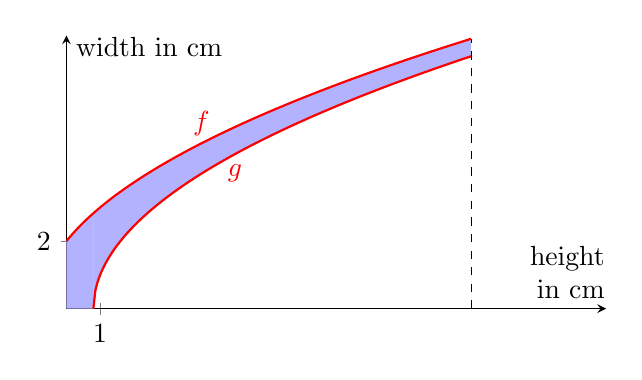
\begin{tikzpicture}
\begin{axis}[
    xlabel={height in cm},
    ylabel={width in cm},
    xmin=0, xmax=16,
    ymin=0, ymax=8.1,
    xtick={1}, ytick={2},
    axis lines=left,
    unit vector ratio=1 1,  % ensure axes use same scale
]
    \addplot [name path=f, red, thick, domain=0:\domainxmax, samples=201] {sqrt(5*x + 4)};
    \addplot [name path=g, red, thick, domain=\gmin:\domainxmax, samples=201] {sqrt(5*x - 4)};
    \path [name path=xaxis]
        (\pgfkeysvalueof{/pgfplots/xmin}, 0) --
        (\pgfkeysvalueof{/pgfplots/xmax}, 0);
    \addplot [blue!30] fill between [
        of=f and g,
        soft clip={domain=\gmin:\domainxmax},
    ];
    \addplot [blue!30] fill between [
        of=f and xaxis,
        % domain is slightly too big to cover initial fill and not leave any gaps
        soft clip={domain=0:\gminepsilon},
    ];
    \node [color=red] at (4, 5.5) {$f$};
    \node [color=red] at (5, 4) {$g$};

    % height from external calulation of f(\domainxmax)
    \draw [dashed] (\domainxmax, 0) -- (\domainxmax, 8.0);
\end{axis}
\end{tikzpicture}

\end{document}
